\subsection*{Problèmes bornés}
\textbf{Problème de Dirichlet:}\\
\underline{Onde:}
\begin{equation*}
    \left\{
    \begin{aligned}
         & u_{tt}=c^2u_{xx} \\
         & u(0,t)=u(l,t)=0  \\
         & u(x,0)=\phi(x)   \\
         & u_t(x,0)=\psi(x)
    \end{aligned}
    \right.
\end{equation*}
\begin{empheq}[box=\fbox]{gather*}
    u(x,t)=\sum_{n=1}^{\infty}\left[A_n\cos\left(\frac{n\pi c}{l}t\right)+B_n\sin\left(\frac{n\pi c}{l}t\right)\right]\sin\left(\frac{n\pi}{l}x\right) \\
    \phi(x)=\sum_{n=1}^{\infty}A_n\sin\left(\frac{n\pi}{l}x\right) \\
    \psi(x)=\sum_{n=1}^{\infty}\frac{n\pi c}{l}B_n\sin\left(\frac{n\pi}{l}x\right)
\end{empheq}
\underline{Diffusion:}
\begin{equation*}
    \left\{
    \begin{aligned}
         & u_t=ku_{xx}     \\
         & u(0,t)=u(l,t)=0 \\
         & u(x,0)=\phi(x)
    \end{aligned}
    \right.
\end{equation*}
\begin{empheq}[box=\fbox]{gather*}
    u(x,t)=\sum_{n=1}^{\infty}A_ne^{-\left(\frac{n\pi}{l}\right)^2kt}\sin\left(\frac{n\pi}{l}x\right) \\
    \phi(x)=\sum_{n=1}^{\infty}A_n\sin\left(\frac{n\pi}{l}x\right)
\end{empheq}
\textbf{Problème de Neumann:}\\
\underline{Onde:}
\begin{equation*}
    \left\{
    \begin{aligned}
         & u_{tt}=c^2u_{xx}    \\
         & u_x(0,t)=u_x(l,t)=0 \\
         & u(x,0)=\phi(x)      \\
         & u_t(x,0)=\psi(x)
    \end{aligned}
    \right.
\end{equation*}
\begin{empheq}[box=\fbox]{gather*}
    \begin{split}
        u(x,t) &=  \frac{1}{2}A_0+\frac{1}{2}B_0t\\
        & +\sum_{n=1}^{\infty}\left[A_n\cos\left(\frac{n\pi c}{l}t\right)+B_n\sin\left(\frac{n\pi c}{l}t\right)\right]\cos\left(\frac{n\pi}{l}x\right)
    \end{split}\\
    \phi(x)=\frac{1}{2}A_0+\sum_{n=1}^{\infty}A_n\cos\left(\frac{n\pi}{l}x\right) \\
    \psi(x)=\frac{1}{2}B_0+\sum_{n=1}^{\infty}\frac{n\pi c}{l}B_n\cos\left(\frac{n\pi}{l}x\right)
\end{empheq}
\underline{Diffusion:}
\begin{equation*}
    \left\{
    \begin{aligned}
         & u_t=ku_{xx}         \\
         & u_x(0,t)=u_x(l,t)=0 \\
         & u(x,0)=\phi(x)
    \end{aligned}
    \right.
\end{equation*}
\begin{empheq}[box=\fbox]{gather*}
    u(x,t)=\frac{1}{2}A_0+\sum_{n=1}^{\infty}A_ne^{-\left(\frac{n\pi}{l}\right)^2kt}\cos\left(\frac{n\pi}{l}x\right) \\
    \phi(x)=\frac{1}{2}A_0+\sum_{n=1}^{\infty}A_n\cos\left(\frac{n\pi}{l}x\right)
\end{empheq}
\textbf{Valeurs propres et fonctions propres:}\\
\underline{Exemple:}\\
Résoudre avec les conditions Dirichlet:
\begin{equation*}
    u_t=ju_{xx}
\end{equation*}
\begin{figure}[H]
    \centering
    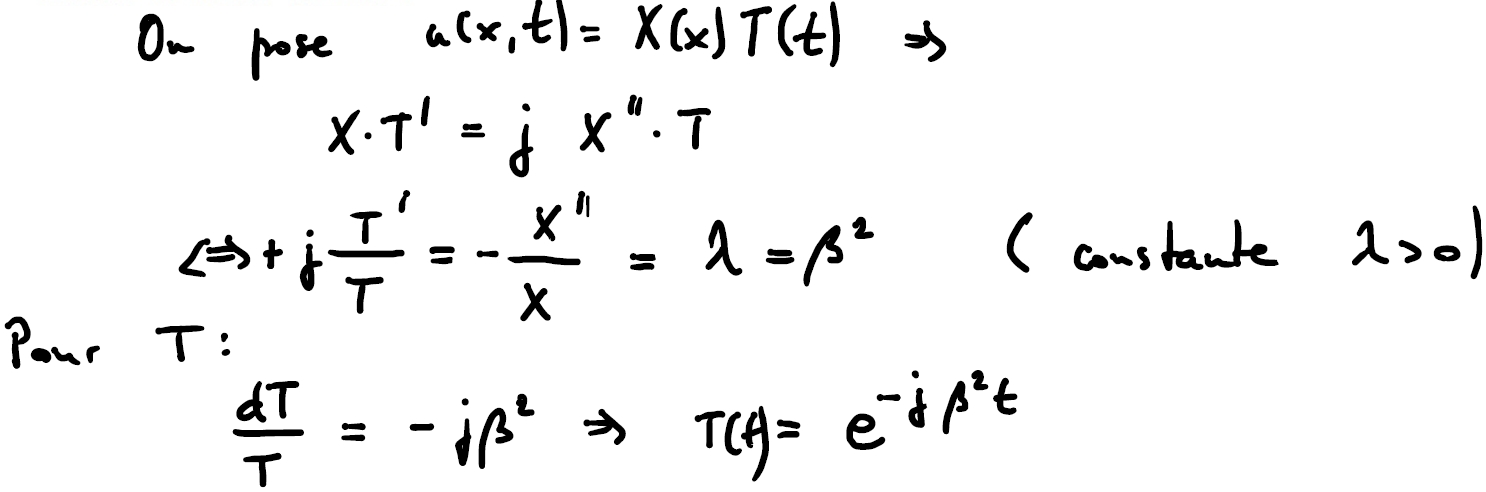
\includegraphics[width=\linewidth]{images/semaine4_val_vect_propre1.png}
\end{figure}
\begin{figure}[H]
    \centering
    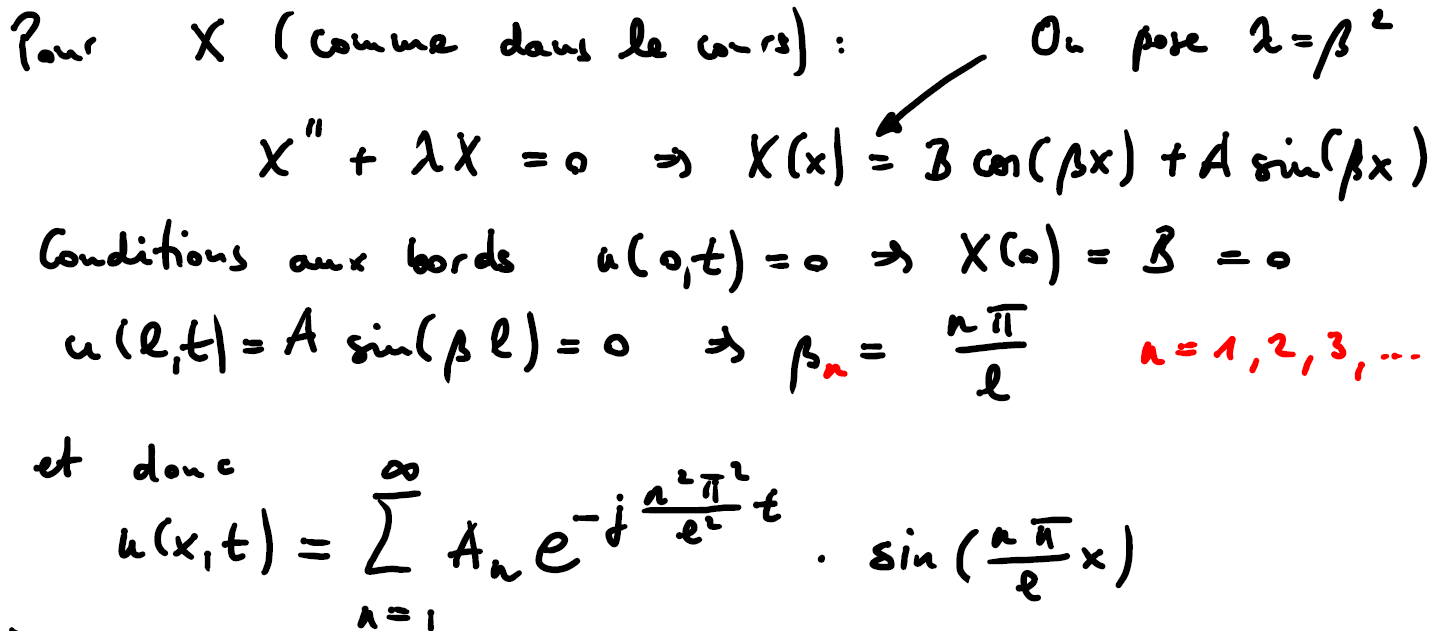
\includegraphics[width=\linewidth]{images/semaine4_val_vect_propre2.png}
\end{figure}
Dans ce cas-ci, la valeur propre est $\lambda=\beta^2=\frac{n^2\pi^2}{l^2}$ trouvée en
résolvant $\frac{-X''}{X}=\lambda$ et la fonction propre est $T(t)=e^{-j\beta^2t}$
trouvée en résolvant $j\frac{T'}{T}=\lambda$.\\
\underline{Conditions mixte}\\
\begin{equation*}
    \lambda=\frac{(n+\sfrac{1}{2})^2\pi^2}{l^2}
\end{equation*}
La fonction propre est elle à calculer selon les conditions au bord spécifiées.\\

